\documentclass[border=5pt]{standalone}
\usepackage{tikz}
\usetikzlibrary{decorations.pathreplacing}
\usepackage{xcolor}

\definecolor{Garnet}{HTML}{73000A}
\definecolor{NinetyBlack}{HTML}{363636}
\definecolor{SeventyBlack}{HTML}{5C5C5C}
\definecolor{FiftyBlack}{HTML}{A2A2A2}
\definecolor{ThirtyBlack}{HTML}{C7C7C7}
\definecolor{Atlantic}{HTML}{466A9F}
\definecolor{Horseshoe}{HTML}{65780B}

\tikzset{every node/.append style={rounded corners=0pt}}

\begin{document}
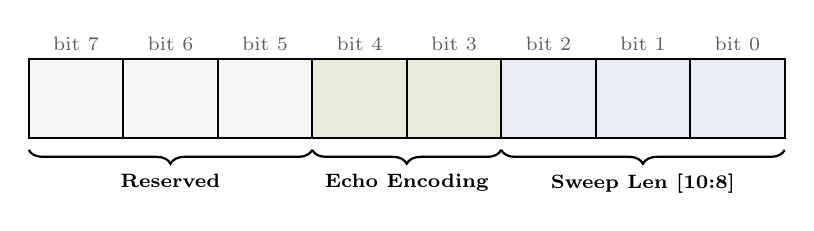
\begin{tikzpicture}

% Bit position labels
\foreach \i/\v in {0/7, 1/6, 2/5, 3/4, 4/3, 5/2, 6/1, 7/0} {
    \node[font=\scriptsize, color=SeventyBlack] at (0.6 + \i*1.2, 1.7) {bit \v};
}

% 8 bit cells
\foreach \i in {0,...,7} {
    \draw[thick] (0 + \i*1.2, 0.5) rectangle (1.2 + \i*1.2, 1.5);
}

% Fills — Reserved bits 7:5
\fill[ThirtyBlack!15] (0, 0.5) rectangle (3.6, 1.5);
\draw[thick] (0, 0.5) rectangle (1.2, 1.5);
\draw[thick] (1.2, 0.5) rectangle (2.4, 1.5);
\draw[thick] (2.4, 0.5) rectangle (3.6, 1.5);

% Fills — Encoding bits 4:3
\fill[Horseshoe!15] (3.6, 0.5) rectangle (6.0, 1.5);
\draw[thick] (3.6, 0.5) rectangle (4.8, 1.5);
\draw[thick] (4.8, 0.5) rectangle (6.0, 1.5);

% Fills — Sweep Len bits 2:0
\fill[Atlantic!12] (6.0, 0.5) rectangle (9.6, 1.5);
\draw[thick] (6.0, 0.5) rectangle (7.2, 1.5);
\draw[thick] (7.2, 0.5) rectangle (8.4, 1.5);
\draw[thick] (8.4, 0.5) rectangle (9.6, 1.5);

% Braces below
\draw[decorate, decoration={brace, amplitude=5pt, mirror}, thick]
    (0, 0.35) -- (3.6, 0.35) node[midway, below=5pt, font=\scriptsize\bfseries] {Reserved};
\draw[decorate, decoration={brace, amplitude=5pt, mirror}, thick]
    (3.6, 0.35) -- (6.0, 0.35) node[midway, below=5pt, font=\scriptsize\bfseries] {Echo Encoding};
\draw[decorate, decoration={brace, amplitude=5pt, mirror}, thick]
    (6.0, 0.35) -- (9.6, 0.35) node[midway, below=5pt, font=\scriptsize\bfseries] {Sweep Len [10:8]};


\end{tikzpicture}
\end{document}
